\documentclass[11pt,a4paper]{article}
\usepackage{amsmath}
\usepackage{amsfonts}
\usepackage{amssymb}
\usepackage{fancyhdr}
\usepackage{lastpage}
\usepackage{graphicx}
\usepackage{ucs}
\usepackage[utf8x]{inputenc}
\usepackage[italian]{babel}

\renewcommand{\headrulewidth}{0.6pt}
\renewcommand{\footrulewidth}{0.6pt}
% impostazione dello stile per le pagine interne del documento
\lhead{\leftmark}
\chead{}
\rhead{
\includegraphics[scale=0.15]{logo.png} }
\lfoot{Analisi dei requisiti v0.5.0}
\cfoot{}
\rfoot{\thepage \ di \pageref{LastPage}}
% ridefinizione dello stile plain per il frontespizio
\fancypagestyle{plain}{
\fancyhf
}
% impostazione dello stile per l'indice
\fancypagestyle{indice}{
\lhead{\leftmark}
\chead{}
\rhead{
\includegraphics[scale=0.15]{logo.png}}
\lfoot{Analisi dei requisiti v0.5.0}
\cfoot{}
\rfoot{}
}
\headheight = 46pt
%definizione del comando "\modifiche" per la creazione del diario delle modifiche
\newcommand{\modifiche} 
{
\newpage
\begin{center}
\textbf{Diario delle modifiche} \\
\bigskip
\begin{tabular}{|c|c|p{0.51\textwidth}|}
\hline
\textsc{Data} & \textsc{Versione} & \textsc{Modifica} \\
\hline
\hline
\textit{2 dicembre 2008} & 0.5.0 & Stesura degli use case \\
\hline
\textit{1 dicembre 2008} & 0.4.1 & Correzione dei requisiti \\
\hline
\textit{30 novembre 2008} & 0.4.0 & Stesura dei requisiti \\
\hline
\textit{29 novembre 2008} & 0.3.0 & Inizio stesura della descrizione del prodotto \\
\hline
\textit{28 novembre 2008} & 0.2.0 & Stesura dell'introduzione \\
\hline
\textit{28 novembre 2008} & 0.1.0 & Stesura dell'indice \\
\hline
\end{tabular}
\end{center}
}
%definizione del comando "\info" per la creazione delle informazioni del documento
\newcommand{\info} {
\bigskip
\begin{tabbing}
	\hspace*{0.3\textwidth} \= \hspace*{0.5\textwidth} \kill
	\parbox{0.3\textwidth}{\textbf{Verifica: }} \> \parbox{0.5\textwidth}{Verificatore} \\
	\parbox{0.3\textwidth}{\textbf{Approvazione: }} \> \parbox{0.5\textwidth}{Responsabile} \\
	\parbox{0.3\textwidth}{\textbf{Stato: }} \> \parbox{0.5\textwidth}{Preliminare} \\
	\parbox{0.3\textwidth}{\textbf{Uso: }} \> \parbox{0.5\textwidth}{Esterno} \\
	\parbox{0.3\textwidth}{\textbf{Distribuzione: }} \> \parbox{0.5\textwidth}{QuiXoft} \\
\end{tabbing}
}
%definizione del comando "\frontespizio" per la creazione del frontespizio
\newcommand{\frontespizio} {
\thispagestyle{plain}
\title{\begin{Huge}\textsc{Progetto SIGEOL}\end{Huge} \\ \textit{Analisi dei requisiti \\ v0.5.0}}
\author{Redazione: Beggiato Andrea, Scarpa Davide, Barbiero Mattia }
\maketitle
\medskip
\begin{center}

\includegraphics[scale=0.5]{logo.png} \\
\textit{quixoft.sol@gmail.com}
\end{center}
\medskip
\info
\newpage
}
%definizione del comando "\indice" per la creazione dell'indice
\newcommand{\indice} {
\thispagestyle{indice}
\tableofcontents
\newpage
}
\pagestyle{fancy}
\begin{document}
\frontespizio
\indice
\setcounter{page}{1}
\section{Introduzione}
\subsection{Scopo del documento}
Il presente documento denominato \textit{Analisi dei requisiti} ha lo scopo di delineare tutti i bisogni espressi dal committente Prof. Rossi Francesca per il sistema \textit{SIGEOL}, nonchè tutti i requisiti intrinsechi nello sviluppo di un tale prodotto. 
\subsection{Scopo del prodotto}
Il progetto sotto analisi, denominato \textit{SIGEOL}, si prefigge di automatizzare la generazione, la gestione, l'ottimizzazione e la consultazione degli orari di lezione. Il committente richiede l'applicazione del sistema al solo corso di laurea in informatica, ma, constatato che la complessità non aumenta notevolmente, il team QuiXoft prevede lo sviluppo e la messa in opera dell'applicazione per tutti i corsi di laurea dell' Università degli studi di Padova.

Il prodotto sarà implementato come un servizio web portabile, facilmente manutenibile ed accessibile agli utenti da una qualsiasi postazione con accesso alla rete Internet.
\subsection{Glossario}
Le definizioni dei termini specialistici usati nella stesura di questo e di tutti gli altri documenti possono essere trovate nel documento ''Glossario'' al fine di eliminare ogni ambiguità e di facilitare la comprensione dei temi trattati. Ogni termine la cui definizione è disponibile all’interno del Glossario verrà marcato con una \underline{sottolineatura}.
\subsection{Riferimenti}
\begin{itemize}
 \item Capitolato d'appalto reperibile all'indirizzo: \\ http://www.math.unipd.it/~tullio/IS-1/2008/Progetti/SIGEOL.html
 \item Statuto di Ateneo reperibile all'indirizzo \\ http://www.unipd.it/organizzazione/statuto/statuto.htm
 \item Informativa sulla privacy (Legge per il trattamento dei dati personali)
 \item Incontri con il committente
\end{itemize}

\section{Descrizione generale}
\subsection{Contesto d'uso del prodotto}
\subsubsection{Processi produttivi e modalità d'uso}
Il funzionamento del sistema \textit{SIGEOL}, a processo produttivo concluso, sarà in grado di guidare ogni singolo utilizzatore (confronta sezione \ref{utenti}) allo svolgimento delle proprie azioni (confronta sezione \ref{funzioni}). In altre parole sarà disponibile un servizio che offrirà, dopo un'opportuna autenticazione, un insieme di strumenti che permetteranno l'inserimento guidato dei dati che serviranno al fine ultimo di generare un orario per le lezioni.
\subsubsection{Piattaforma d’esecuzione ed interfacciamento con l’ambiente di installazione e uso}
Il prodotto sarà realizzato tramite un'applicazione web supportata da un database e dovrà essere accessibile da un qualsiasi tipo di browser. Data la mancanza di un applicativo preesistente al quale aggiungere le funzioni del sistema \textit{SIGEOL}, il team QuiXoft dovrà definirne ogni aspetto creando un prodotto che sia accessibile, manutenibile, portabile e soprattutto sicuro. A tal scopo verranno adottate tecnologie gratuite e moderne per lo sviluppo di pagine dinamiche e sarà necessario disporre di un server affidabile.
\subsection{Funzioni del prodotto} \label{funzioni}

\subsection{Caratteristiche degli utenti} \label{utenti} 
\subsection{Vincoli generali}
\subsection{Assunzioni e dipendenze}
\section{Requisiti}
\subsection{Requisiti funzionali}
\subsubsection{Requisiti funzionali per la segreteria generale}
\begin{itemize}
\item \textbf{OBBLIGATORI}
\begin{enumerate}
\item Possibilità di login/logout
\item Possibilità di inserimento delle facoltà
\item Possibilità di invitare via e-mail le singole facoltà ad inserire i dati
\item Possibilità di consultare lo schema d'orario di ogni corso di laurea
\end{enumerate}
\item \textbf{DESIDERABILI}
\begin{enumerate}
\item Possibilità di impostare la frequenza con cui avviene il backup automatico dei dati
\end{enumerate}
\end{itemize}
\subsubsection{Requisiti funzionali per la segreteria didattica}
\begin{itemize}
\item \textbf{OBBLIGATORI}
\begin{enumerate}
\item Possibilità di login/logout
\item Possibilità di inserimento e modifica, all'interno della propria facoltà, per ogni corso, del nome, dei relativi CFU, dell'anno di appartenenza, del periodo, dello stato, del numero di ore in aula e in laboratorio (se previsto), del docente di riferimento che lo tiene, di eventuali assistenti e della stima del numero di studenti che lo seguiranno
\item Possibilità di inserimento e modifica, all'interno della propria facoltà, per ogni aula disponibile, del nome, della capienza, delle ore e dei periodi di non disponibilità
\item Possibilità di inserimento e modifica dell'anno accademico
\item Possibilità di inserimento e modifica delle ore da usare
\item Possibilità di impostare linee guida per la creazione dell'orario
\item Possibilità di modifica dei dati dei docenti preventivamente inseriti dal Presidente del CCS
\item Possibilità di invitare via e-mail i presidenti del CCS di ogni corso di laurea ad inserire i dati
\end{enumerate}
\item \textsc{DESIDERABILI}
\begin{enumerate}
\item Possibilità di generazione dello schema d'orario in formato pdf e html
\item Possibilità di scegliere vincoli da rilassare e soluzioni subottime, proposti dal sistema, in caso di soluzione inesistente
\item Possibilità di consultare lo schema d'orario di ogni corso di laurea della propria facoltà
\end{enumerate}
\end{itemize}
\subsubsection{Requisiti funzionali per il Presidente del CCS}
\begin{itemize}
\item \textbf{OBBLIGATORI}
\begin{enumerate}
\item Possibilità di login/logout
\item Possibilità di inserimento e modifica, all'interno del proprio corso di laurea, per ogni corso, del nome, dei relativi CFU, dell'anno di appartenenza, del periodo, dello stato, del numero di ore in aula e in laboratorio (se previsto), del docente di riferimento che lo tiene, di eventuali assistenti e della stima del numero di studenti che lo seguiranno
\item Possibilità di inserimento e modifica, all'interno del proprio corso di laurea, per ogni aula disponibile, del nome, della capienza, delle ore e dei periodi di non disponibilità
\item Possibilità di inserimento e modifica, all'interno del proprio corso di laurea, dei nomi e delle e-mail dei docenti
\item Possibilità di inserimento e modifica dell'anno accademico
\item Possibilità di inserimento e modifica delle ore da usare
\item Possibilità di impostare linee guida per la creazione dell'orario
\item Possibilità di generazione dello schema d'orario in formato pdf e html
\item Possibilità di scegliere vincoli da rilassare e soluzioni subottime, proposti dal sistema, in caso di soluzione inesistente
\item Possibilità di consultare lo schema d'orario
\item Possibilità di inserimento di vincoli e preferenze relativi ai corsi
\item Possibilità di inserimento e modifica di indirizzi diversi appartenenti allo stesso corso di laurea
\end{enumerate}
\item \textbf{DESIDERABILI}
\begin{enumerate}
\item Possibilità di notificare il mancato inserimento di un docente o di un corso d'insegnamento di un altro corso di laurea
\item Possibilità di impostare una data limite per l'inserimento dei vincoli da parte dei docenti, con segnalazione della scadenza via e-mail
\item Possibilità di modifica manuale dello schema d'orario specificato
\end{enumerate}
\end{itemize}
\subsubsection{Requisiti funzionali per i docenti}
\begin{itemize}
\item \textsc{OBBLIGATORI}
\begin{enumerate}
\item Possibilità di inserimento e modifica dei propri giorni e ore di indisponibilità, con relativa motivazione
\item Possibilità di inserimento e modifica delle proprie preferenze su orari e giorni di lezione, con relativa motivazione
\item Possibilità di modifica dei propri dati personali
\end{enumerate}
\end{itemize}
\subsection{Requisiti di qualità}
\begin{itemize}
\item \textbf{OBBLIGATORI}
\begin{enumerate}
\item Accessibilità del sistema
\item Garanzie sull'integrità dei dati
\item Gestione in sicurezza degli account
\item Manutenibilità del sistema
\item Interfaccia utente semplice e intuitiva
\item Presenza di manuali d'uso, di installazione, configurazione e manutenzione del sistema
\item Il prodotto dovrà essere consegnato assieme ad un ambiente di prova per verificarne il corretto funzionamento
\end{enumerate}
\item \textbf{DESIDERABILI}
\begin{enumerate}
\item Portabilità del sistema
\item Completa interoperabilità dei dati memorizzati e trattati
\item Pagine scritte in XHTML e CSS dovranno essere validate tramite strumenti forniti dal consorzio W3C
\end{enumerate}
\end{itemize}
\subsection{Requisiti d'interfacciamento e d'ambiente}
\subsubsection{Con l’ambiente di installazione ed uso}
\begin{itemize}
\item \textbf{OBBLIGATORI}
\begin{enumerate}
\item Le informazioni andranno memorizzate in modo permanente in una base di dati
\end{enumerate}
\item \textbf{DESIDERABILI}
\begin{enumerate}
\item Le tecnologie da adottare dovranno essere gratuite
\end{enumerate}
\end{itemize}
\subsubsection{Con l’operatore}
\begin{itemize}
\item \textbf{OBBLIGATORI}
\begin{enumerate}
\item Le informazioni dovranno essere acquisite tramite un servizio web
\item Il sistema distinguerà i vari tipi di utente tramite autenticazione
\item Al fine di evitare errori il sistema dovrà il più possibile proporre all'utente i dati in modo automatico
\end{enumerate}
\end{itemize}
\section{Use case e descrizioni narrative}
In questo capitolo verranno illustrati i diagrammi use-case che rappresentano
i requisiti funzionali del prodotto. 

I diagrammi verrano accompagnati dalle loro descrizioni narrative per consentirne
una migliore comprensione.
\subsection{Use case generale}
Il seguente diagramma illustra in modo generale le funzionalità offerte dal sistema SIGEOL.
\begin{center}
 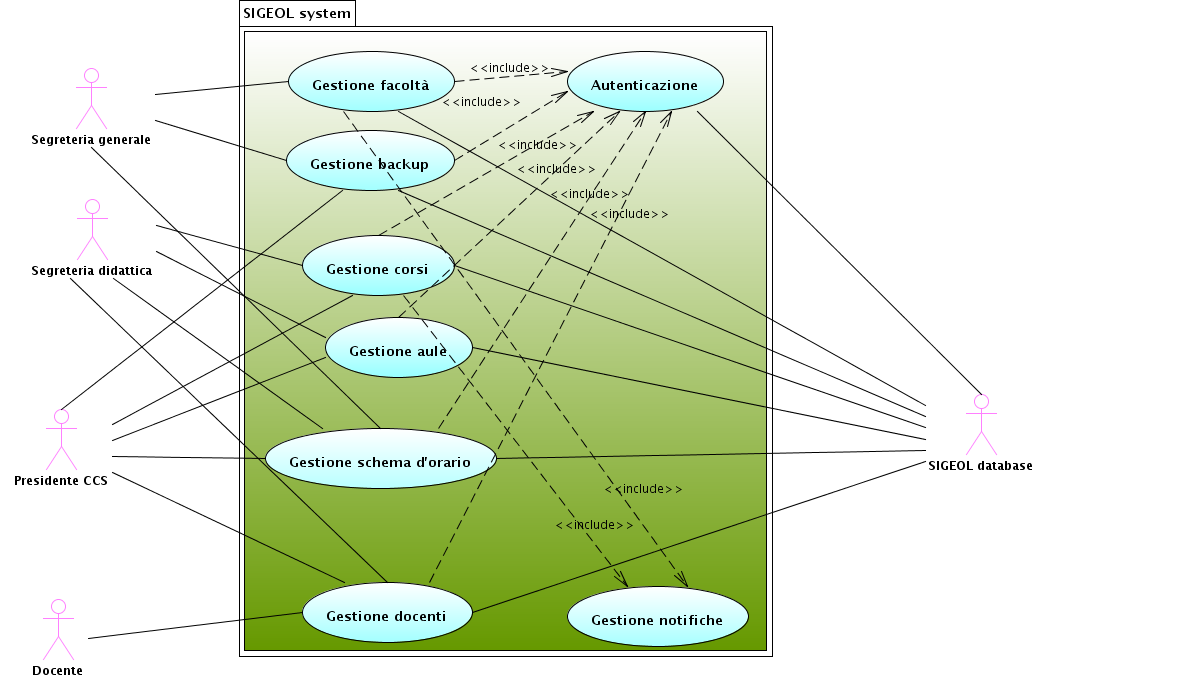
\includegraphics[scale=0.7]{UseCaseSistema.png}
 % UseCaseSistema.png: 638x495 pixel, 72dpi, 22.51x17.46 cm, bb=0 0 638 495
\end{center}

Il sistema è composto da otto parti principali:
\begin{enumerate}
\item Gestione facoltà: modulo per la gestione dei dati relativi alle facoltà. 
\item Gestione corsi: modulo per la gestione dei dati relativi ai corsi.
\item Gestione aule: modulo per la gestione dei dati relativi alle aule.
\item Gestione docenti: modulo per la gestione dei dati relativi ai docenti.
\item Gestione schema d'orario: modulo per la gestione e la generazione dello schema d'orario.
\item Gestione backup: modulo per la gestione dei backup del SIGEOL database.
\item Autenticazione: modulo utilizzato per autenticare le varie tipologie di utenti.
\item Gestione notifiche: modulo per la gestione delle notifiche.
\end{enumerate}
\textbf{Attori coinvolti:}
Segreteria generale, segreteria didattica, presidente CCS, docente

\subsection{Use case Gestione facoltà}
\begin{center} 
 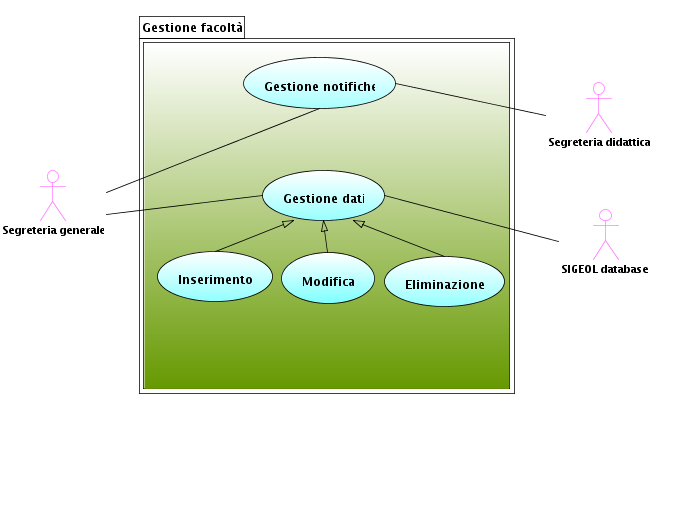
\includegraphics[scale=0.7]{UseCaseGestioneFacolta.png}
 % UseCaseGestioneFacolta.png: 801x496 pixel, 72dpi, 28.26x17.50 cm, bb=0 0 801 496
\end{center}

\subsubsection*{Attori coinvolti:}
Segreteria generale.

\subsubsection*{Scopo e descrizione sintetica:}
L'utente 'Segreteria generale' inserisce, modifica ed elimina i dati relativi alle facoltà universitarie.

\subsubsection*{Pre-condizioni:}
L'utente 'Segreteria generale' accede dalla sua pagina personale alla sezione 'Gestione facoltà'.

\subsubsection*{Flusso base di eventi:}
\begin{enumerate}
 \item L'utente inserisce una nuova facoltà.
 \item L'utente invia una notifica alla segreteria didattica della facoltà inserita.
\end{enumerate}

\subsubsection*{Flussi alternativi:}
\begin{enumerate}
 \item L'utente modifica i dati di una facoltà precedentemente inserita.
 \item L'utente elimina una facoltà.
 \item L'utente ritorna alla sua pagina personale
\end{enumerate}

\subsubsection*{Post-condizioni:}
Le modifiche relative alle facoltà vengon oinserite nel SIGEOL database e le notifiche vengono correttamente 
inviate alle varie segreterie didattiche.

\subsection{Use case Gestione corsi}
\subsection{Use case Gestione aule}
\subsection{Use case Gestione docenti}
\subsection{Use case Gestione schema d'orario}
\subsection{Use case Gestione backup}
\subsection{Use case Autenticazione}
\subsection{Use case Gestione notifiche}
\modifiche
\end{document}
